
%----------------------------------------------------------------------
% SECTION Hardware PCB
%----------------------------------------------------------------------
\section{Hardware Design}
\label{sec:Hardware Design}

In diesem Unterkapitel wird die Entwicklung der Hardware für den MVB-Sniffer beschrieben. Zu den Kernkomponenten zählen der RS485-Transceiver SP3485CN-L/TR, das FPGA 10M08SAE144C8G und der Mikrocontroller ESP32-S3-WROOM-1. Die Hauptaufgabe besteht darin, die Funktionalitäten der drei Evaluationsboards zu analysieren und die Bauteile auf die für die Anwendung als MVB-Sniffer notwendigen Komponenten zu reduzieren. Dabei wurde auch berücksichtigt, welche zusätzlichen Funktionen in der weiteren Entwicklung von Nutzen sein könnten. Ziel ist, ein für den Anwendungszweck optimiertes PCB-Design (Printed Circuit Board) zu erstellen, das alle wesentlichen Anforderungen für die Signalverarbeitung und -analyse erfüllt und die verschiedenen elektronischen Bauteile und Chips in einem kompakten Design vereint. Im Rahmen dieser Arbeit wurde zunächst ein Schema erstellt, welches als Grundlage für die spätere Entwicklung des PCB dient. Als Software wurde hierfür Altium verwendet. Die Abbildung \ref{fig:Hardware Übersicht} zeigt ein vereinfachtes Blockschaltbild, wie die Komponenten zusammen verbunden sind. Das System wird per Micro USB mit Spannung versorgt und besitzt über 3 DC/DC-Wandler. Für das FPGA  ein Wandler von 5 V auf 3.3 V, für den ESP32-S3 und den RS485 ebenfalls ein Wandler von 5 V auf 3.3 V und für die Referenzspannung des FPGA ein Wandler von 3.3 V auf 2.5 V. Nachfolgend werden die zentralen Funktionen anhand von Ausschnitten aus dem Schema detailliert erläutert. Das gesamte Schema ist in PDF-Format im Anhang \ref{app:Schemata} aufzufinden, sowie die Stückliste dazu \ref{app:bom.pdf}.

\begin{figure}[H]
    \centering
    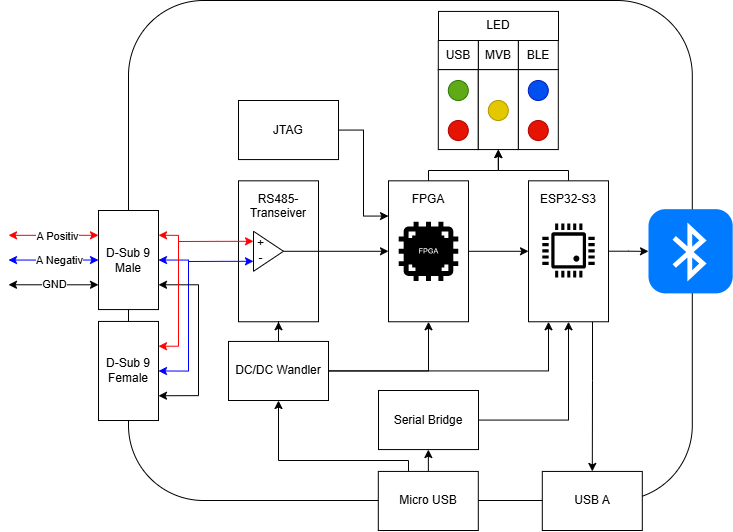
\includegraphics[width=0.8\linewidth]{Figures/Chap3/Schematics/Aufbau_Hardware_Sniffer.drawio.png}
    \caption{Hardware Übersicht}
    \label{fig:Hardware Übersicht}
\end{figure}


\subsection{RS485-Transceiver}

Wie in Abbildung \ref{fig:MVB to RS485} ersichtlich, wird das MVB-Signal durch den Sniffer über die beiden D-Sub-Stecker J1 und J2 durchgeführt und abgegriffen. Anschliessend wird es zum RS485-Transceiver SP3485CN-L/TR weitergeleitet. Der RS485-Transceiver verarbeitet die differentiellen Signale des MVB \textit{Data P} und \textit{Data N}. Er wandelt diese in ein einheitliches Signal \textit{MVB Data} um, das für die Weiterverarbeitung durch den FPGA verwendet wird. Dabei werden lediglich die 3 Leitungen der Linie A des MVB-Signals analysiert, während die redundante Linie B nicht abgegriffen wird (Pin 4 und Pin 5 des D-Sub-Steckers), da sie in Fahrzeugen in der Praxis selten verwendet wird. Die Pins \textit{DI}, $\overline{RE}$ und \textit{DE} werden mit dem \textit{GND} gelegt, um sicherzustellen, dass der Sniffer nur als Empfänger fungiert. Durch diese Konfiguration ist der Treiber deaktiviert (\textit{DE} auf \textit{GND}) und der Empfänger aktiviert ($\overline{RE}$ auf \textit{GND}), sodass das Gerät nur Daten vom MVB empfangen kann, ohne selbst Daten auf den Bus zu senden. Dies verhindert, dass der Datenverkehr auf dem Bus unbeabsichtigt beeinflusst wird. Die weiteren Pin Funktionen sind aus der Tabelle \ref{tab:pin_funktionen} zu entnehmen. Das Datenblatt befindet sich im Anhang \ref{app:File51}.

\begin{figure}[H]
    \centering
    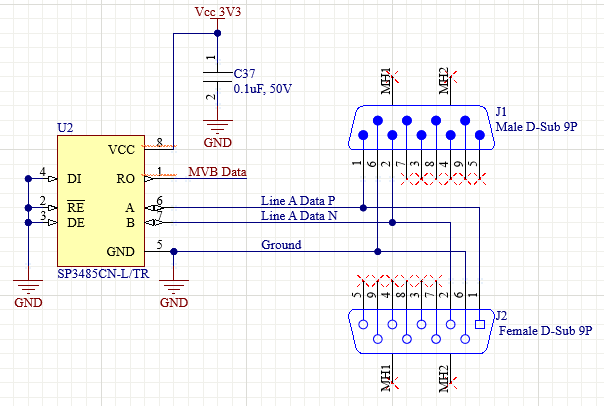
\includegraphics[width=0.8\linewidth]{Figures/Chap3/Schematics/MVB to RS485.png}
    \caption{Vom MVB Signal zum RS485}
    \label{fig:MVB to RS485}
\end{figure}

\begin{table}[h]
  \centering
  \begin{tabular}{|c|c|l|}
    \hline
    \textbf{Pin} & \textbf{Funktion} & \textbf{Beschreibung} \\ \hline
    1 & RO & Receiver Output \\ \hline
    2 & $\overline{\text{RE}}$ & Receiver Output Enable Active LOW \\ \hline
    3 & DE & Driver Output Enable \\ \hline
    4 & DI & Driver Input \\ \hline
    5 & GND & Ground Connection \\ \hline
    6 & A & Driver Output/Receiver Input Non-inverting \\ \hline
    7 & B & Driver Output/Receiver Input Inverting\\ \hline
    8 & Vcc & Versorgungsspannung \\ \hline
  \end{tabular}
  \caption{Beschreibung der Pin-Funktionen}
  \label{tab:pin_funktionen}
\end{table}

\textcolor{red}{Datenblatt SP3485CN-L/TR} 

\subsection{FPGA}
Ein FPGA ist ein flexibler Chip, der aus programmierbaren Logikblöcken, I/O-Banken und Verbindungsnetzwerken besteht. Die Konfiguration entscheidet, welche Funktionen der FPGA übernimmt und wie die einzelnen Blöcke und Schnittstellen zusammenarbeiten. Der 10M08SAE144C8G verfügt über 8 Banken, die unterschiedlich konfiguriert werden können. Für die Anwendung im MVB-Sniffer wurde nur die Hälfte der Banken verwendet, jedoch alle 8 Banken mit Spannung versorgt, um für die Weiterentwicklung flexibel zu sein und um Störungen oder unerwartetes Verhalten zu vermeiden. 

\subsubsection{Programmierung}

Programmiert wird der FPGA über die JTAG-Schnittstelle (Joint Test Action Group). Das ist ein standardisiertes Protokoll zur Programmierung, Konfiguration und Debuggen von elektronischen Bausteinen wie Mikrocontrollern oder FPGA. Über die JTAG-Signale \textit{TCK} (Test Clock), \textit{TMS} (Test Mode Select), \textit{TDI} (Test Data Input) und \textit{TDO} (Test Data Output) können Daten seriell übertragen werden. Das Signal \textit{JTAGEN} (JTAG Enable) aktiviert die JTAG-Funktion. Im FPGA wird die Bank 1B für die JTAG-Schnittstelle verwendet, die eine zentrale Rolle bei der Konfiguration des FPGA spielt. Dies konnte vom Evaluationsboard übernommen werden, da dieses so programmiert wird. Es sind zwei Modi möglich:

\begin{enumerate}
    \item Direkte Konfiguration über .sof-Dateien:
    Mithilfe des JTAG-Steckers kann eine .sof-Datei direkt in das FPGA geladen werden. Diese Datei enthält die Informationen für die momentane Programmierung des FPGA. Dabei wird der FPGA bei einem Neustart oder einer erneuten Konfiguration in einen leeren Zustand versetzt, da die Konfiguration nur temporär gespeichert wird.
    \item Programmierung der Configuration Flash Memory (CFM) mit .pof-Dateien: 
    Alternativ kann über den JTAG-Header eine .pof-Datei in das CFM des FPGA programmiert werden. In diesem Fall startet der FPGA nach jedem Neustart automatisch in den Selbstkonfigurationsmodus und lädt die gespeicherten Daten aus dem CFM.
\end{enumerate}

\begin{figure}[H]
    \centering
    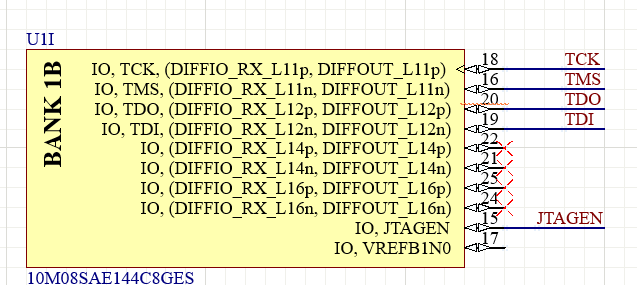
\includegraphics[width=1.0\linewidth]{Figures/Chap3/Schematics/Bank1B_JTAG.png}
    \caption{FPGA Bank 1B: JTAG}
    \label{FPGA JTAG}
\end{figure}

Wie in Abbildung \ref{FPGA JTAG} ersichtlich, ist die JTAG-Schnittstelle der Stecker \textit{J6}, welche mit einem USB-Blaster verbunden werden kann. Die 10 kOhm Widerstände sorgen dafür, dass die Signale \textit{TCK}, \textit{TMS} und \textit{JTAGEN} auf logisch \textit{"1"} gehalten werden, wenn sie nicht aktiv angesteuert werden. Dies verhindert Fehlfunktionen durch unbestimmte Pegel. Der 1 kOhm Widerstand hält \textit{TDI} auf logisch \textit{"0"}, wenn kein Signal anliegt, auch um ungewollte Signalpegel zu vermeiden. Somit werden die Signale über die Pins des Steckers \textit{J6} mit dem FPGA verbunden, \textit{JTAGEN} wird auf logisch \textit{"1"} gezogen, wodurch das FPGA in den Programmierungsmodus versetzt wird und über die restlichen Pins die Programmdaten und Steuersignale an das FPGA sendet.


\subsubsection{Oszillator}

Es wird analog zum Evaluationsboard der Oszillator CB3LV-3C-50M0000 verwendet, damit ein stabiler und präziser externer Takt von 50 MHz zur Verfügung steht. Dieser Takt wird benötigt, um die Abläufe im FPGA zu synchronisieren und zusätzliche Takte zu erzeugen, die es für bestimmte Aufgaben braucht. Dafür wird der Oszillator mit einem dedizierten Clock-Pin des FPGA auf Bank 2 verbunden (siehe Abbildung \ref{FPGA OSC}).

\begin{figure}[H]
    \centering
    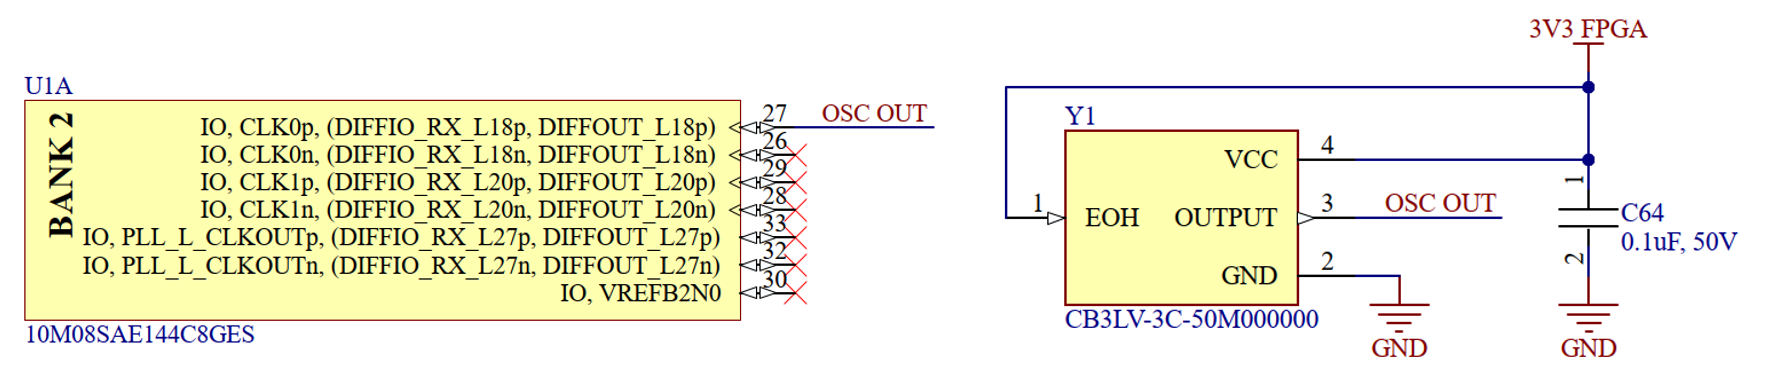
\includegraphics[width=1.0\linewidth]{Figures/Chap3/Schematics/Bank2_OSC.png}
    \caption{FPGA Bank 2: Oszillator}
    \label{FPGA OSC}
\end{figure}

\subsubsection{Steuersignale}
\label{subsec:Steuersignale}

Auf der Bank 8 des FPGA gibt es mehrere Steuersignale, die in der zukünftigen Anwendung von wichtiger Bedeutung sein können (siehe Abbildung \ref{FPGA Admin}).

\begin{itemize}
    \item Durch das Betätigen des Knopfes S4 wird das FPGA gezwungen, sich aus dem Configuration Flash Memory (CFM) neu zu konfigurieren, indem das \textit{NCONFIG} Signal vom FPGA auf das \textit{GND} Potenzial gezogen wird. Da in Zukunft die Programmierung über die CFM laufen soll, erscheint diese Funktion als wichtig.
    
    \item Das Betätigen des Knopfes S4 setzt alle Register im FPGA zurück. Dies kann für eine schnelle Rücksetzung des Systems genutzt werden, ohne das FPGA vollständig neu zu konfigurieren. Das Signal \textit{RESET N} wird auf den dafür vorgesehenen Pin auf dem FPGA geführt und beim Drücken vom Knopf S4 auf das \textit{GND} Potenzial gezogen.
    
    \item Mit diesem Schalter SW1 wird ausgewählt, welches CFM-Bild (Konfigurationsbild) beim Start des FPGA verwendet wird, wenn eine Dual-Image-Konfiguration vorliegt. Diese Funktionen ermöglichen eine flexible Konfiguration und Steuerung des FPGA, insbesondere wenn in einem zukünftigen Schritt mehrere Konfigurationsoptionen gefordert werden, wie zum Beispiel eine Umschaltung von ESD auf EMD. Dies geschieht mit dem Steuersignal \textit{BOOT SEL}.
\end{itemize}

\begin{figure}[H]
    \centering
    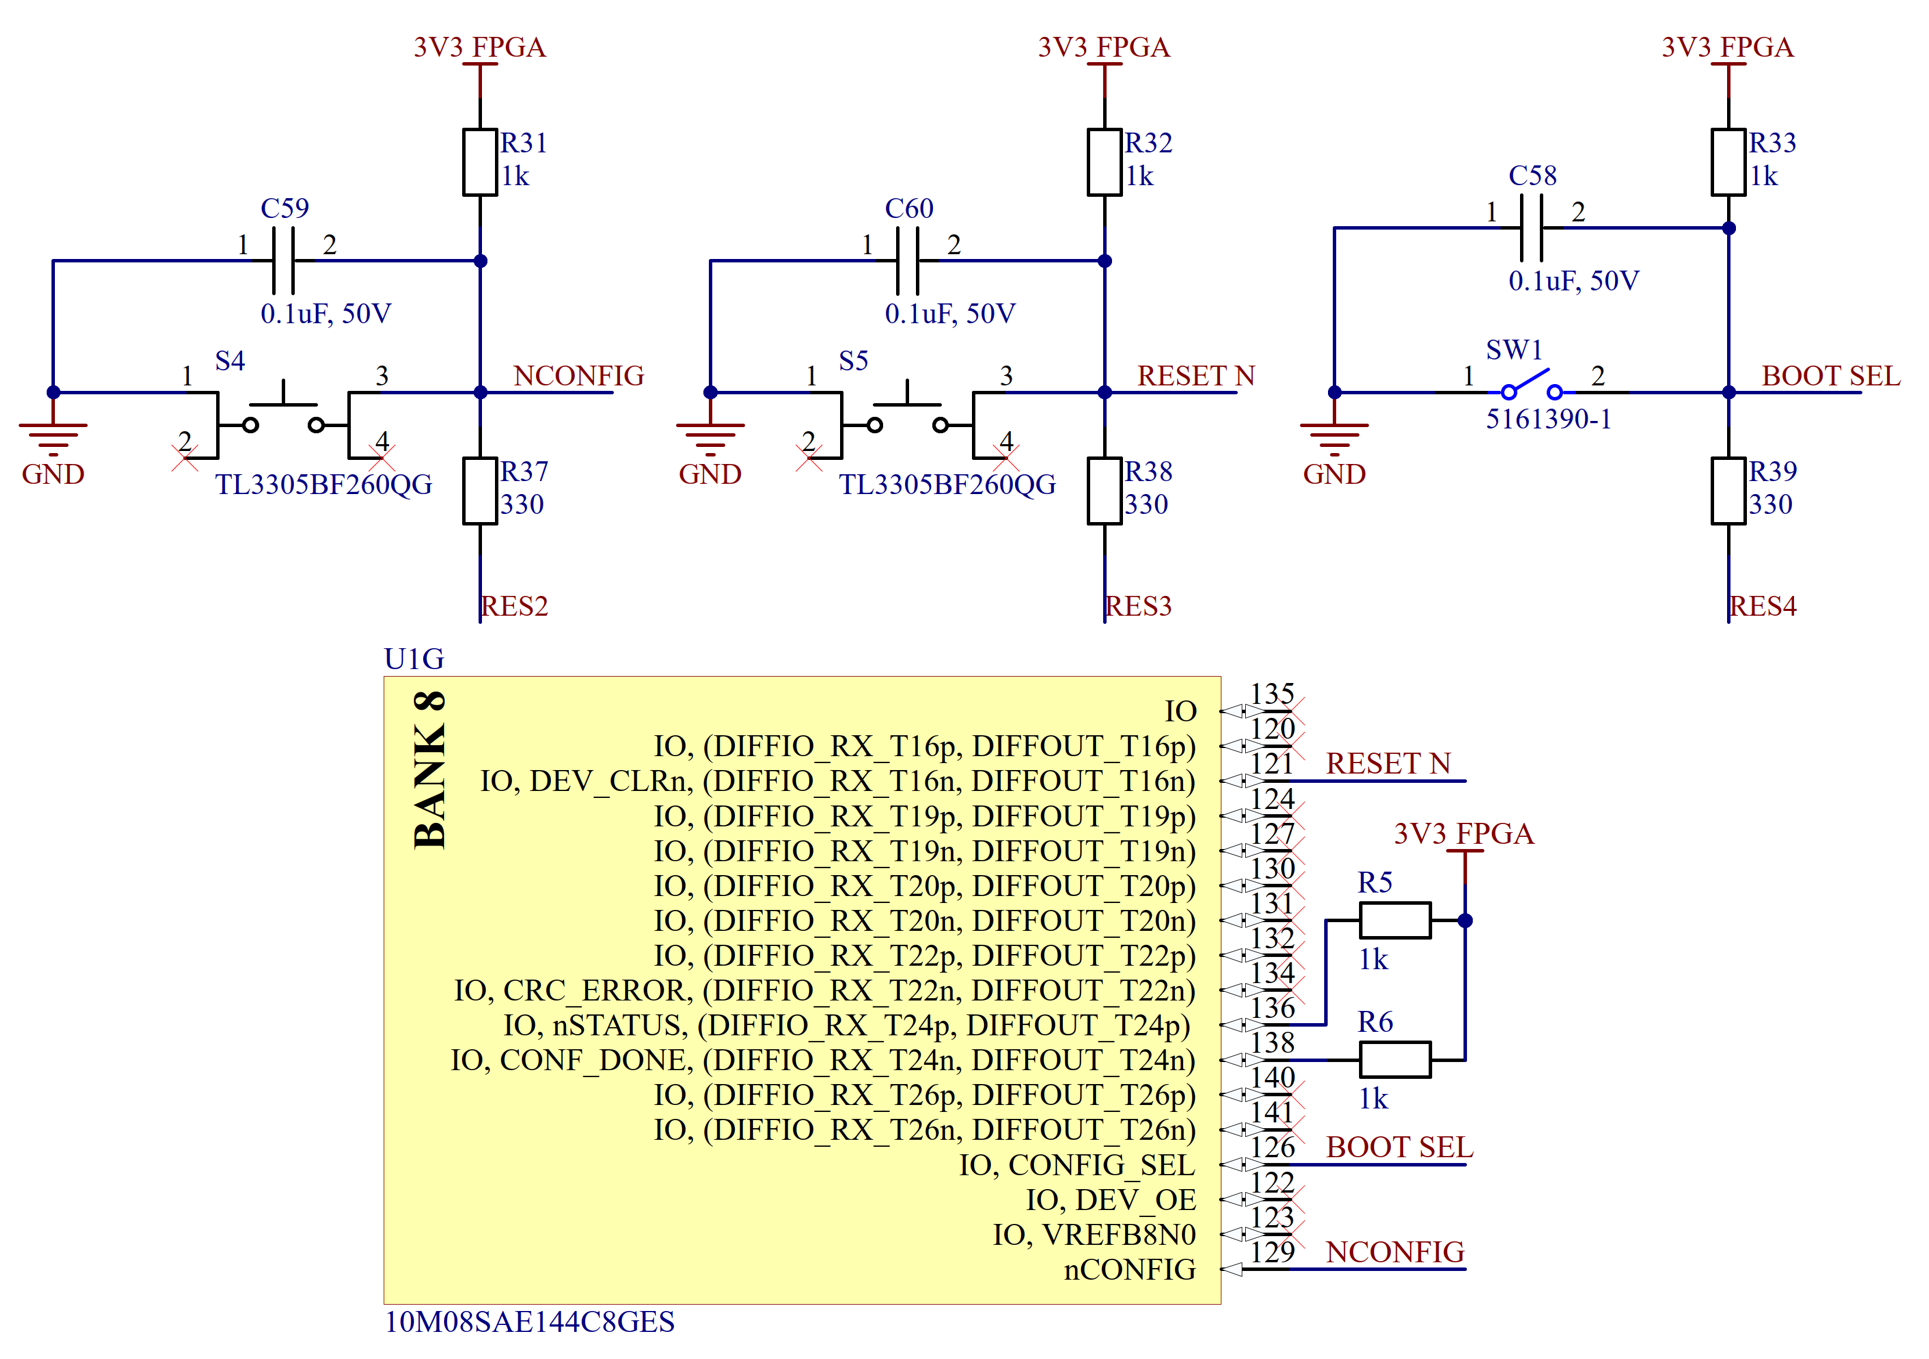
\includegraphics[width=1.0\linewidth]{Figures/Chap3/Schematics/Bank8_Admin.png}
    \caption{FPGA Bank 8: Steuersignale FPGA}
    \label{FPGA Admin}
\end{figure}

Diese drei Steuersignale können auch über die \textit{RES2} bis \textit{RES4} Leitungen vom Mikro Controller ESP32-S3 gesteuert werden. Dies geschieht über die Pull-Down-Widerstände R33 bis R35 und den entsprechenden GPIO vom ESP32, welche die Leitungen auf logisch \textit{"0"} ziehen können.

\subsubsection{Schnittstellen}
\label{subsubsec:Schnittstellen}
Für die Kommunikation zwischen dem FPGA, dem ESP32-S3 und dem RS485 wurde die Bank 3 vorgesehen. In dieser Bank sind die SPI-Signale (\textit{CS, MOSI} und \textit{SCLK}) so verbunden, dass eine direkte Kommunikation zwischen dem FPGA und dem ESP32-S3 ermöglicht wird. Um die Überschwinger zu reduzieren, wurden bereits 0 Ohm Widerstände angedacht, die in Zukunft ersetzt werden können durch grössere Widerstände. Zusätzlich wurde eine Handshake-Leitung \textit{HS FPGA}, Interrupt-Leitung \textit{INTR FPGA} und eine Master In, Slave Out Leitung \textit{MISO} integriert, um künftige Erweiterungen zu vereinfachen.

Darüber hinaus stehen die Reserveleitungen \textit{RES1} bis \textit{RES4} zur Verfügung. Diese Leitungen können neben der Funktion, den FPGA zu steuern, wie im letzten Abschnitt von Kapitel \ref{subsec:Steuersignale}(\textit{RES2} bis \textit{RES4}) beschrieben, auch als zusätzliche Verbindung zwischen FPGA und ESP32-S3 dienen, wo sie noch keine festgelegte Funktion besitzen.

Zusätzlich wurden \textit{FPGA RES5} bis \textit{FPGA RES7} Leitungen angedacht, welche direkt auf eine Pinleiste gehen. Somit kann über einen Steckverbinder künftig die FPGA IO, flexibel und schnell erweitert werden.

Für das Signal \textit{MVB Active} wurde eine LED-Ansteuerung mithilfe eines Darlington-Arrays vorgesehen (Details dazu in Kapitel \ref{subsec:Indikatoren}). Somit soll der Sniffer in Zukunft anzeigen, sobald er MVB Aktivität auf dem RS485 erkennt.

\begin{figure}[H]
    \centering
    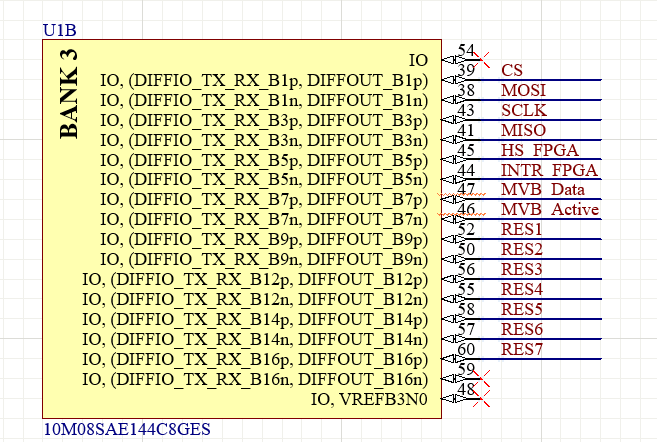
\includegraphics[width=1.0\linewidth]{Figures/Chap3/Schematics/Bank3_ESP.png}
    \caption{FPGA Bank 3: ESP32 Interface}
    \label{FPGA ESP}
\end{figure}

Das Datenblatt sowie das Schema des FPGA Evaluationsboards befinden sich im Anhang \ref{app:File52} (Datenblatt) und \ref{app:File53} (Schema).

\subsection{ESP32-S3}
Der Mikrocontroller ESP32-S3-WROOM-1 unterstützt Bluetooth Low Energy (BLE), WLAN, verfügt über eine hohe Flexibilität bei der Konfiguration der GPIO, einen Dual-Core-Prozessor und bietet eine Vielzahl von Schnittstellen wie SPI, I$^2$C und UART.

\subsubsection{Programmierung}
Die USB-UART-Brücke CP2102N-A02-GQFN28, in Abbildung \ref{fig:UART_Bridge}, ermöglicht die einfache Kommunikation zwischen einem Computer und dem ESP32-S3 Mikrocontroller über die serielle Schnittstelle. Diese UART-Verbindung wird vor allem für das Flashen der Firmware auf den ESP32, sowie für Debugging-Zwecke genutzt. Die Leitungen \textit{USB DP} und \textit{USB DN} kommen von einer Micro-USB-Schnittstelle auf den CP2102N. Von dort gehen die Leitungen \textit{U0RXD} und \textit{U0TXD} dann weiter zum ESP32.

Eine Programmierschaltung ermöglicht eine automatische Umschaltung des ESP32-S3 zwischen Normalmodus (Run) und Programmiermodus (Boot), ohne dass physische Tasten erforderlich sind. Mit dem CP2102N und dessen Steuerleitungen \textit{DTR, RTS} kann der ESP32-S3 in die verschiedenen Modi geschaltet werden. Über eine Transistorschaltung werden diese Leitungen verwendet, um die Pins EN (Reset) und GPIO0 (Boot-Modus) auf dem ESP32-S3 anzusteuern, wie in Abbildung \ref{fig:ESP32_Steuersignale} ersichtlich. Das Gleiche kann auch über die Taster S1 und S2 gemacht werden und der S3 besitzt noch keine Funktion, kann in Zukunft aber beliebig verwendet werden.

\begin{figure}[H]
    \centering
    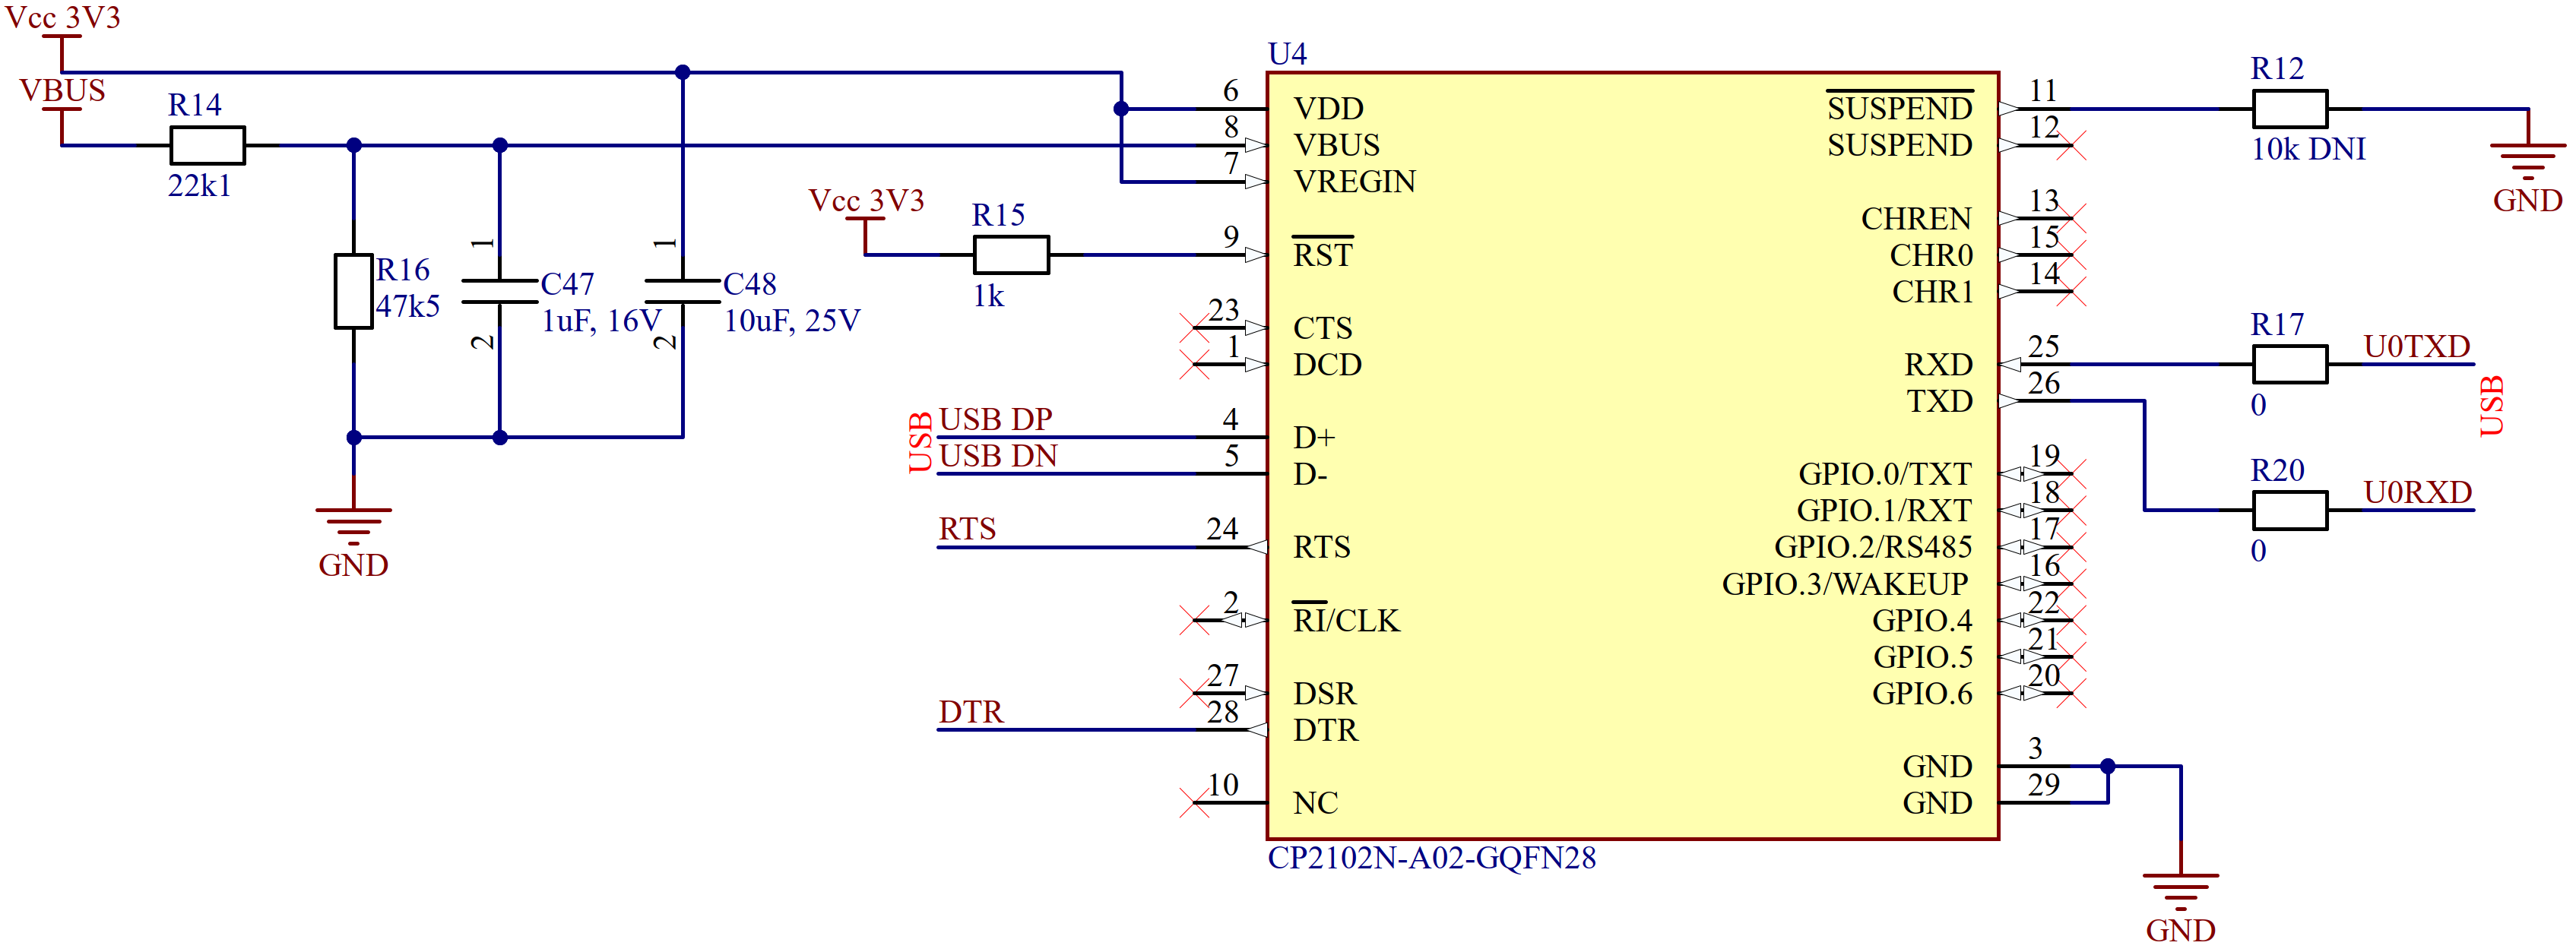
\includegraphics[width=1\linewidth]{Figures/Chap3/Schematics/UART_Bridge.png}
    \caption{USB-UART-Brücke}
    \label{fig:UART_Bridge}
\end{figure}

Das Datenblatt der USB-UART-Brücke CP2102N-A02 befindet sich im Anhang \ref{app:File54}.

\begin{figure}[H]
    \centering
    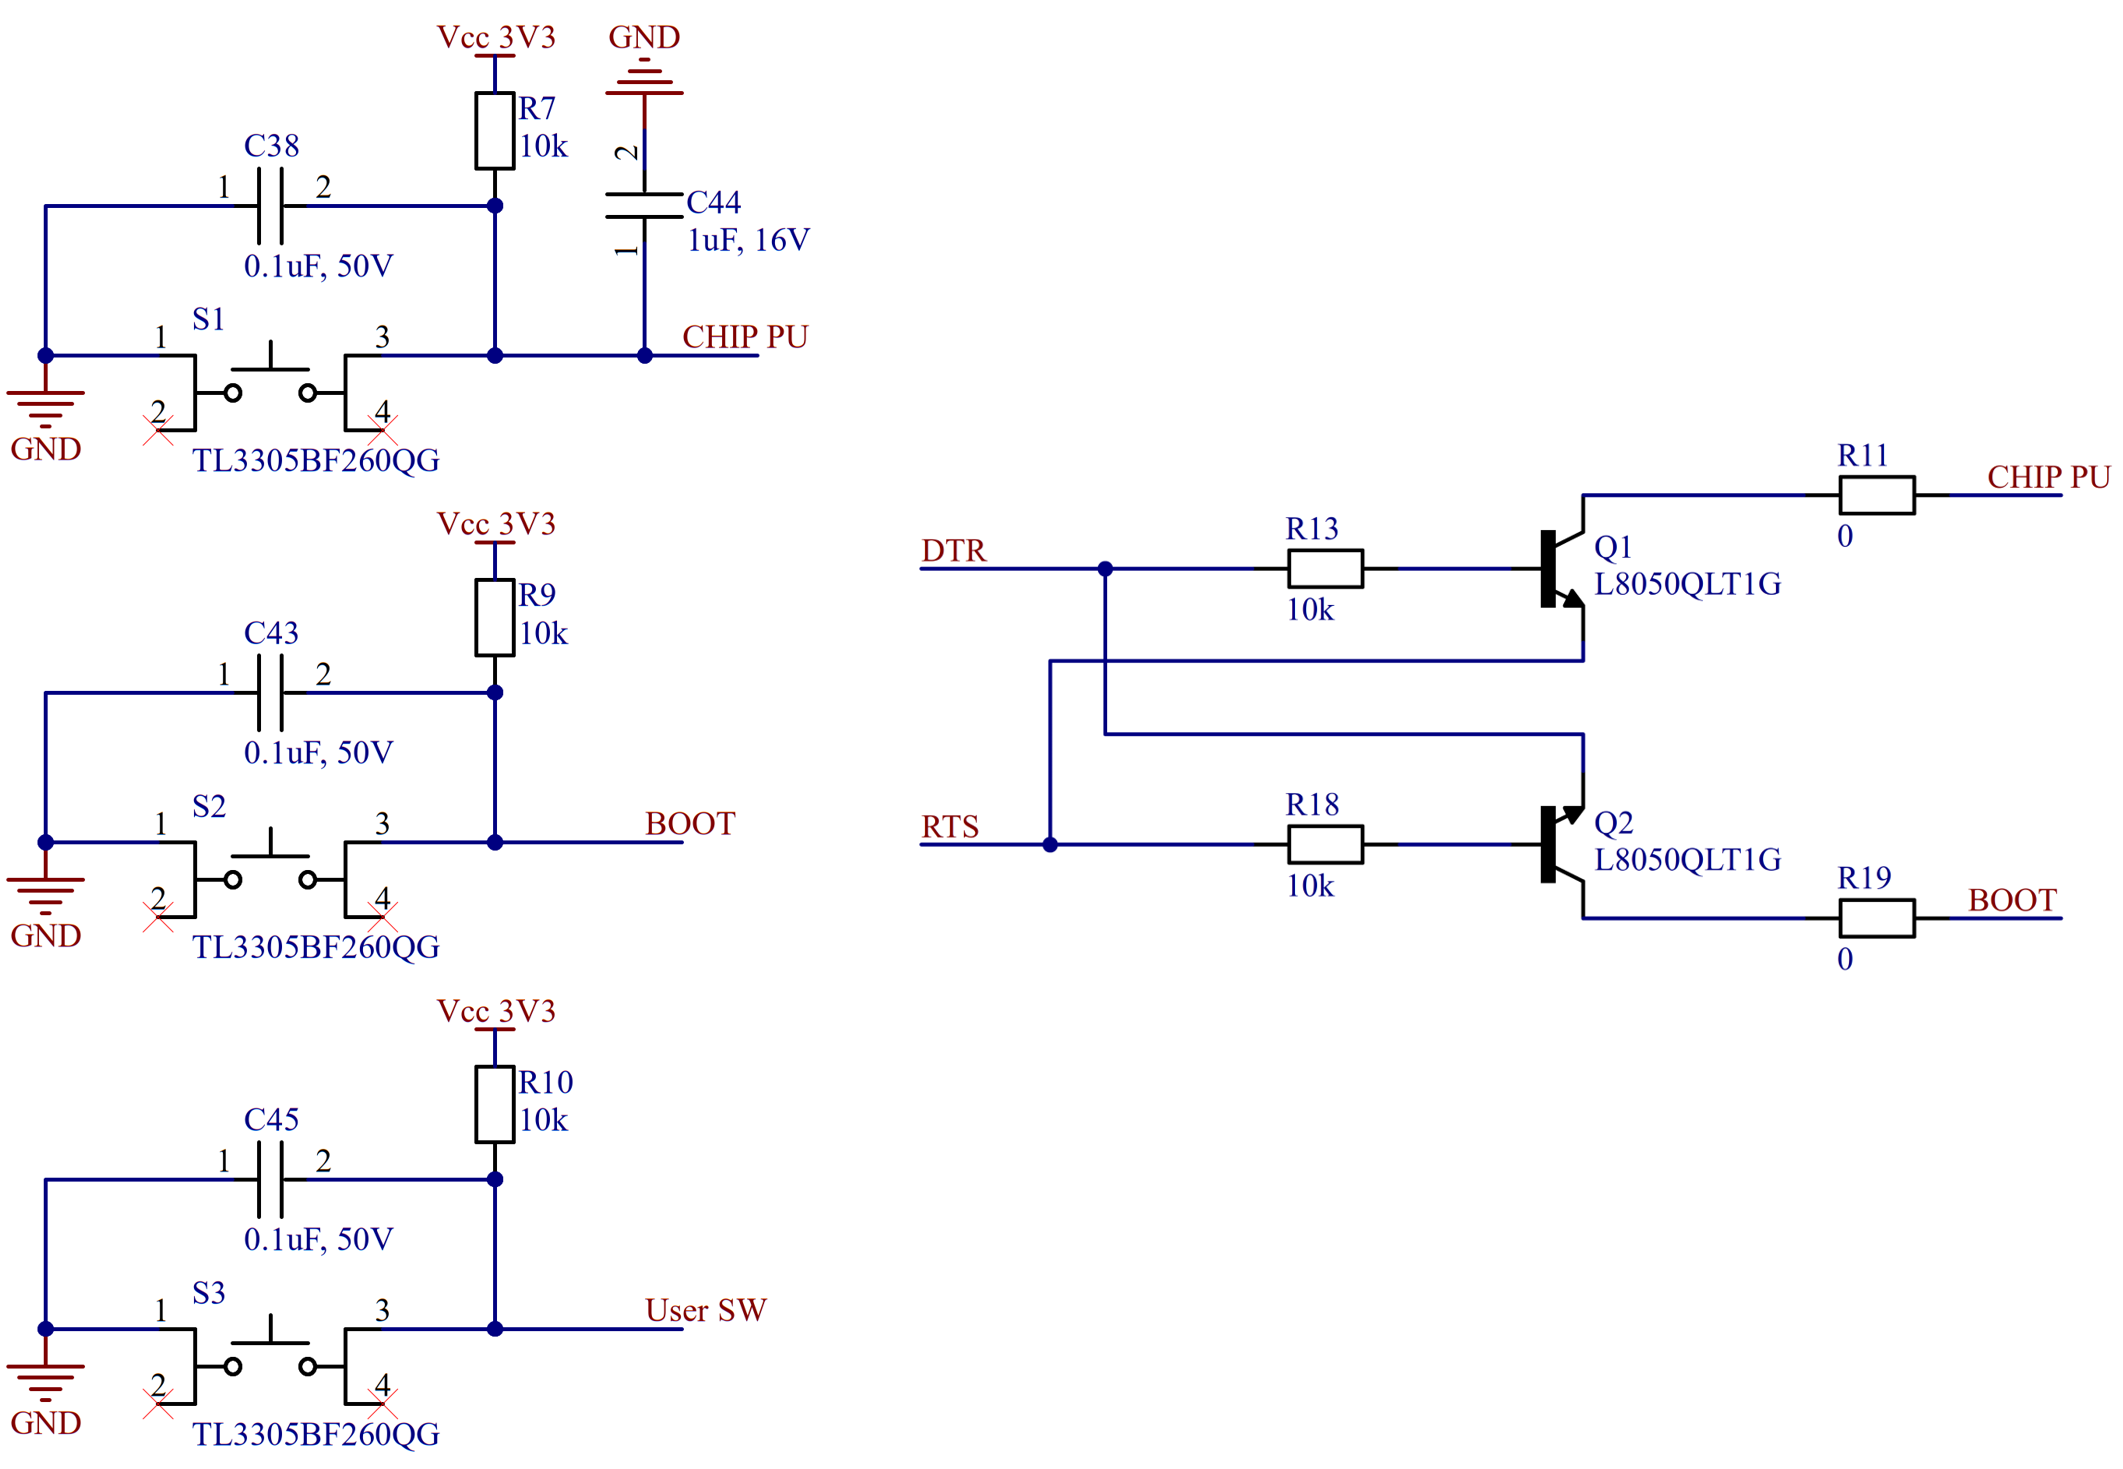
\includegraphics[width=1\linewidth]{Figures/Chap3/Schematics/ESP32_Steuersignale.png}
    \caption{ESP32 Steuersignale}
    \label{fig:ESP32_Steuersignale}
\end{figure}

Normalbetrieb
\textit{DTR} = 1, \textit{RTS} = 1: Beide Transistoren bleiben gesperrt, wodurch EN und GPIO0 auf HIGH liegen. Der ESP32-S3 startet und läuft im Normalmodus.

Programmiermodus:
\textit{DTR} = 0, \textit{RTS} = 1: Der Transistor für GPIO0 (Boot-Pin) wird aktiviert, wodurch GPIO0 auf Low gezogen wird, während EN HIGH bleibt. Der ESP32-S3 wird dadurch in den Flash-Modus versetzt.

Reset:
\textit{DTR} = 1, \textit{RTS} = 0: Der Transistor für EN wird aktiviert, wodurch der Reset-Pin des ESP32-S3 (CHIP PU) auf Low gezogen wird. Dies führt zu einem Neustart des Mikrocontrollers. 

Diese Steuersignale wurden  zusammengefasst in der Tabelle \ref{tab:operation_modes}.
\begin{table}[h]
  \centering
  \begin{tabular}{|c|c|c|c|l|}
    \hline
    DTR & RTS & EN (CHIP PU) & GPIO0 & Modus \\ \hline
    1   & 1   & 1            & 1     & Normalbetrieb (Run) \\ \hline
    0   & 1   & 1            & 0     & Programmiermodus (Boot) \\ \hline
    1   & 0   & 0            & 1     & Reset \\ \hline
  \end{tabular}
  \caption{Operation Modi}
  \label{tab:operation_modes}
\end{table}



\subsubsection{USB-A}
Eine USB-A-Schnittstelle soll ermöglichen, in Zukunft Daten des Sniffers nicht nur per Bluetooth auszugeben, sondern auch über einen USB-Stick zu loggen, sodass man nicht immer mit einem Bluetooth-fähigen Gerät in der Nähe sein muss. Dies geschieht über zwei GPIO des ESP32. Die beiden Leitungen (\textit{USB-A N, USB-A P}) sind direkt mit dem ESP32-S3 verbunden und sind ersichtlich in Abbildung \ref{fig:ESP32}.

\subsubsection{GPIO}
 Die restlichen GPIO des ESP32-S3 in der Abbildung \ref{fig:ESP32} auf die noch nicht eingegangen worden ist, sind zum einen die 7 Leitungen, die LED ansteuern (\textit{BLE LED b, BLE LED r, USB LED g, USB LED r, Akku low, Akku mid, Akku full}). Hierzu folgt mehr in Kapitel \ref{subsec:Indikatoren}. Die Leitung \textit{ADC Akku} wird über einen Spannungsteiler auf dem ADC-Eingang vom ESP32-S3 eingelesen, um den Akkustand zu bestimmen.
 
\begin{figure}[H]
    \centering
    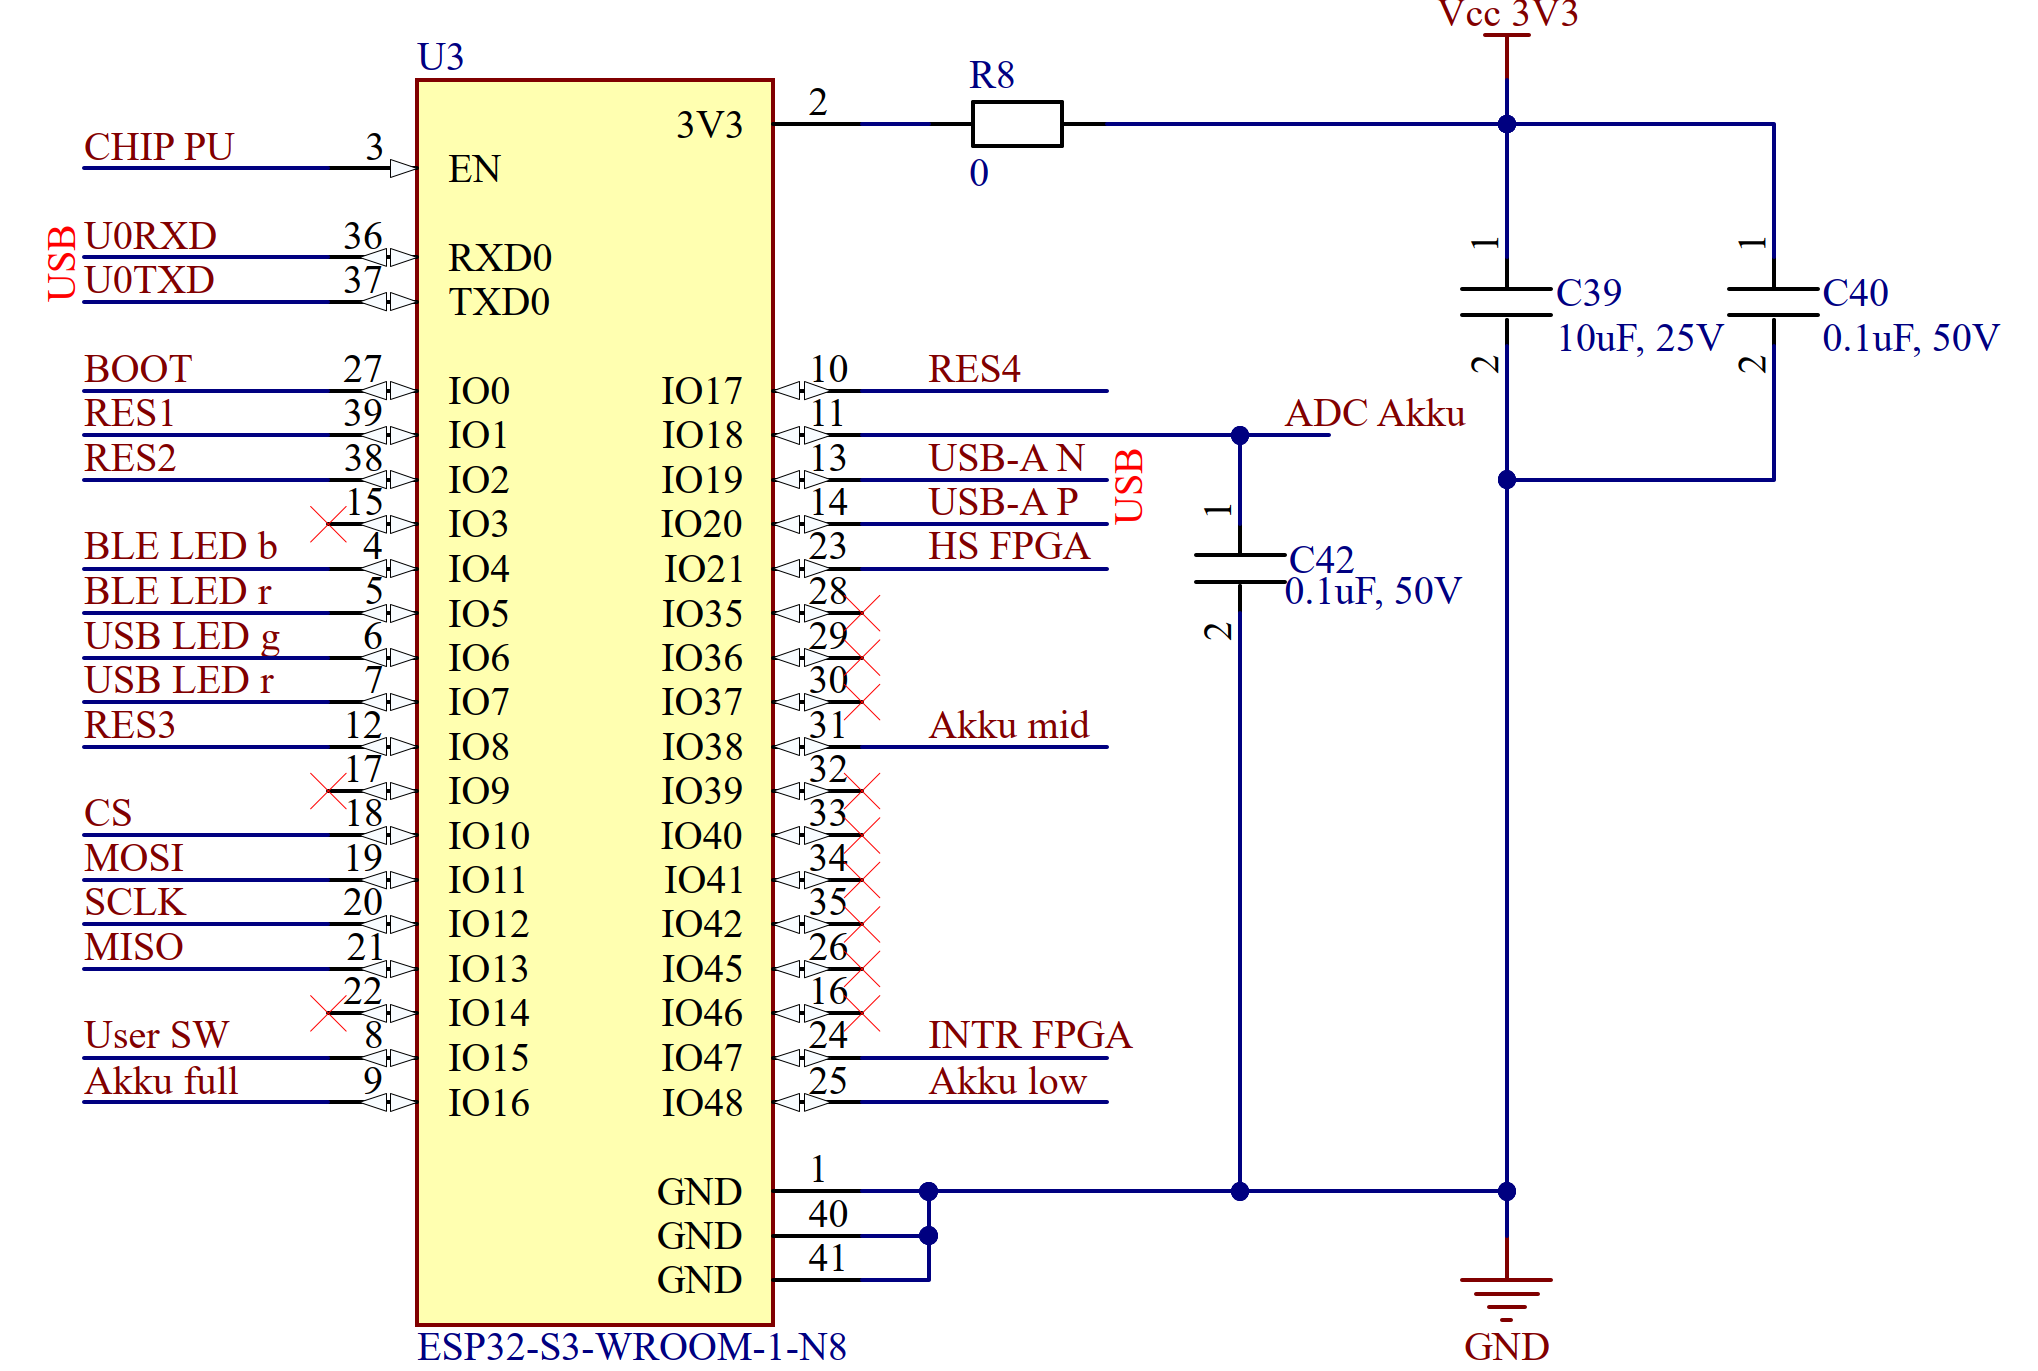
\includegraphics[width=0.8\linewidth]{Figures/Chap3/Schematics/ESP32.png}
    \caption{ESP32-S3}
    \label{fig:ESP32}
\end{figure}

Das Datenblatt sowie das Schema des ESP32-S3 Evaluationsboards befinden sich im Anhang \ref{app:File55} (Datenblatt) und \ref{app:File56} (Schema).

\subsection{Indikatoren}
\label{subsec:Indikatoren}
Zur Anzeige der Betriebszustände der Kommunikationsschnittstellen werden LEDs eingesetzt, die über den Darlington-Array-Transistor ULN2803CDWR vom ESP32-S3 oder FPGA angesteuert werden. Der ULN2803CDWR ermöglicht die Steuerung der LEDs, indem er acht Darlington-Transistorpaare integriert, die eine Stromverstärkung ermöglichen. Im Betrieb wird der Eingang eines Kanals auf HIGH geschaltet, wodurch der zugehörige Ausgang auf GND gezogen wird. Dadurch kann ein Laststrom durch die angeschlossene LED fliessen, welche mit einem Vorwiderstand betrieben wird, um den Strom zu begrenzen. Der Einsatz des ULN2803CDWR ermöglicht somit eine effiziente Steuerung der Statusanzeigen durch die digitalen Ausgänge des ESP32-S3 oder FPGA, ohne die Steuerlogik mit hohen Strömen zu belasten. Die Bluetooth-Schnittstelle wird durch eine blaue und eine rote LED signalisiert, während die USB-Schnittstellen mit einer grünen und einer roten LED dargestellt werden. Eine gelbe LED soll die Aktivität auf dem MVB anzeigen,  sobald der Sniffer angeschlossen wird. Zukünftig ist ein Akkubetrieb vorgesehen, weshalb auch eine Ladezustandsanzeige mittels LEDs eingeplant wurde. 
Das Datenblatt des ULN2803CDWR befindet sich im Anhang \ref{app:File57}.
\begin{figure}
    \centering
    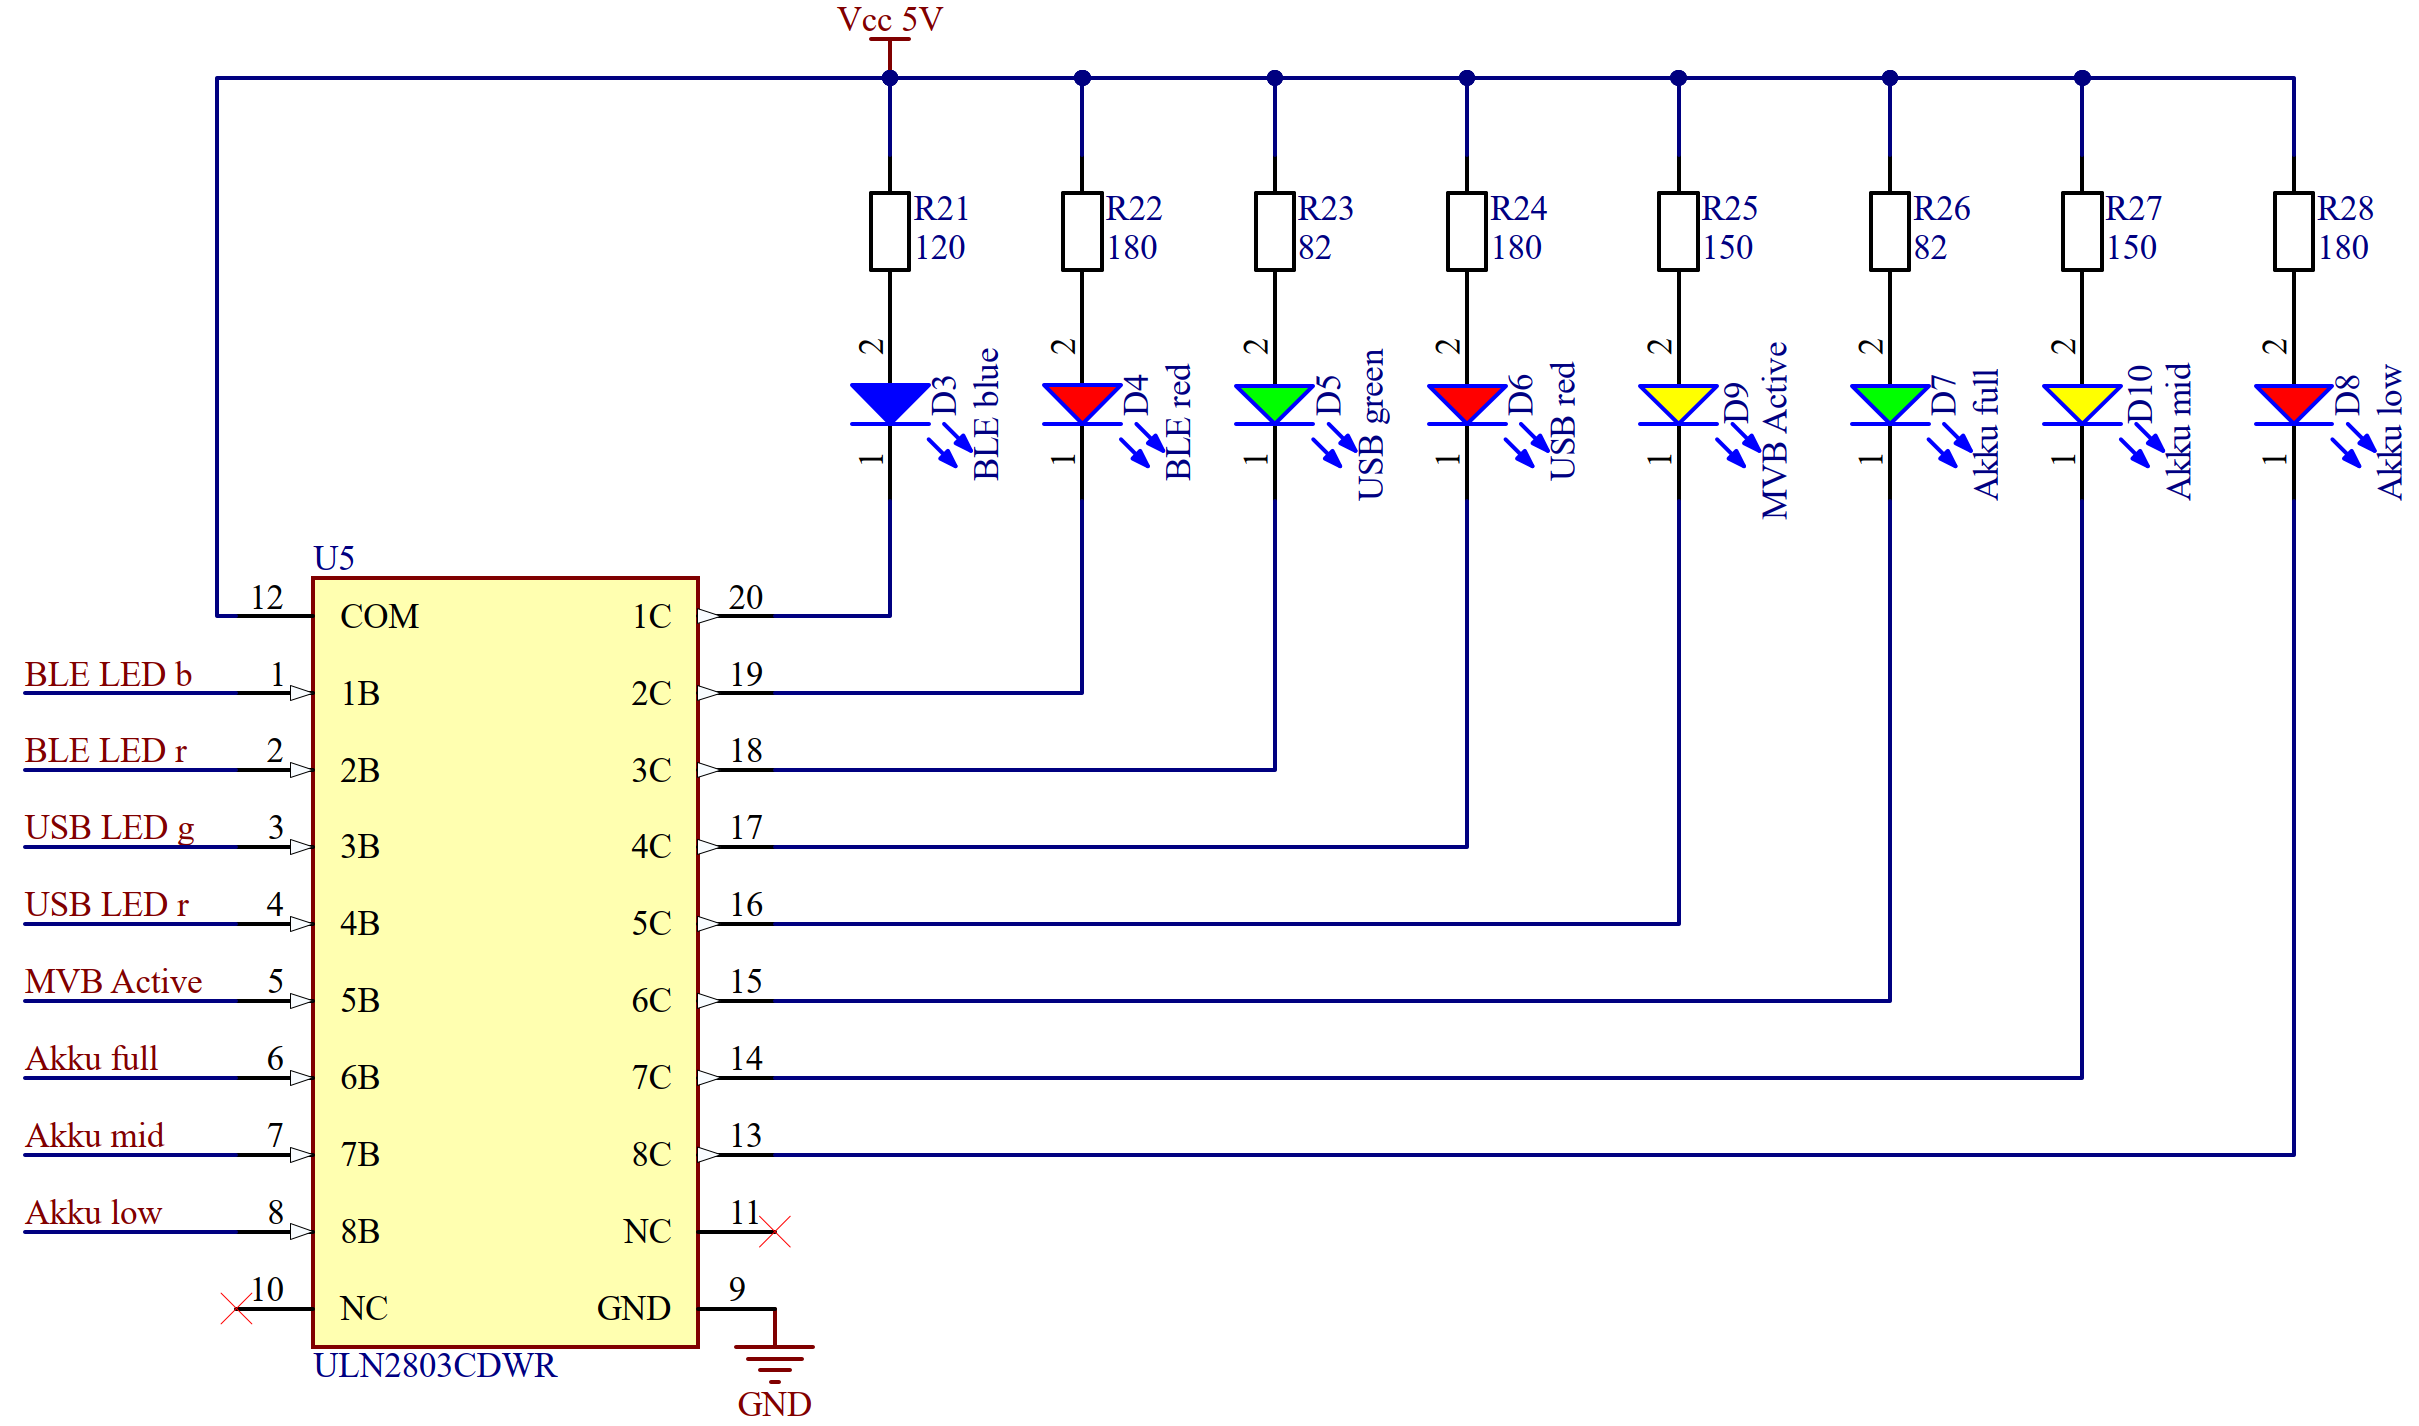
\includegraphics[width=0.9\linewidth]{Figures/Chap3/Schematics/Indicator_LEDs.png}
    \caption{Status LED}
    \label{fig:StateLED}
\end{figure}
